\documentclass{beamer}

\usepackage{url}           % format URLs
\usepackage{listings}      % format code
\lstset{
  mathescape, 
  language={C},
  basicstyle=\small
}
%\usepackage{enumitem}      % adjust spacing in enums
%\usepackage[colorlinks=true,allcolors=blue,breaklinks,draft=false]{hyperref}   
\usepackage{graphicx}
\usepackage{float}
\usepackage{subcaption}
\usepackage{xspace,framed}
\usepackage{colortbl}
\usepackage{calc}
%\usepackage[dvipsnames]{xcolor}
\usepackage{amssymb,amsmath,amsfonts} 
\usepackage{mathtools}
\usepackage{microtype}
\usepackage{epstopdf}


\usepackage{algorithm}
\usepackage{amsfonts}
\usepackage{multicol}
\usepackage{multirow}
\usepackage{tikz}
\usetikzlibrary{positioning, automata, shapes.arrows, calc, shapes, arrows}
\usetikzlibrary{patterns}
\usepackage[justification=centering]{caption}
\usepackage{stmaryrd}
\usepackage{hhline}
\usepackage{pifont}
\usepackage{pgfplots}
\usepackage{longtable}
\usepackage{afterpage}
\usepackage{wasysym}
\usepackage[scaled]{helvet}
\usepackage{mdwlist}

\newtheorem{myassumption}{Assumption}
\newtheorem{mylemma}{Lemma}
\newtheorem{myprop}{Proposition}

\renewcommand{\baselinestretch}{0.991}
\allowdisplaybreaks
\newcommand\tool{{\sf DSSynth}\xspace}
\newcommand{\xmark}{\ding{55}}
\newcommand{\mat}[1]{\boldsymbol{#1}}
\newcommand{\cavslides}[1]{#1}


\begin{document}

\title {Sound and Automated Synthesis of Digital Controllers for Continuous Plants}

\author{\textbf{Alessandro Abate}, Iury Bessa, Dario Cattaruzza, Lucas Cordeiro, Cristina David, Pascal Kesseli and Daniel Kroening}

\date{March 2017}

\frame{\maketitle}

\begin{frame}{Cyber-Physical Systems (CPS)}

\begin{itemize}
\item 
modern controls are implemented with digital microcontrollers, 
embedded within dynamical plants representing physical components 
\item 
digital control literature: success and limitations 
\end{itemize} 

\begin{figure}
    \centering
    \begin{subfigure}[b]{0.3\textwidth}
        \includegraphics[width=\textwidth]{figures/step1_figureB.png}
    \end{subfigure}
    ~
    \begin{subfigure}[b]{0.3\textwidth}
        \includegraphics[width=\textwidth]{figures/step1_figureC.png}
    \end{subfigure}
%     ~
%    \begin{subfigure}[b]{0.3\textwidth}
%        \includegraphics[width=\textwidth]{figures/step1_figureD.png}
%    \end{subfigure}
    ~
    \begin{subfigure}[b]{0.3\textwidth}
        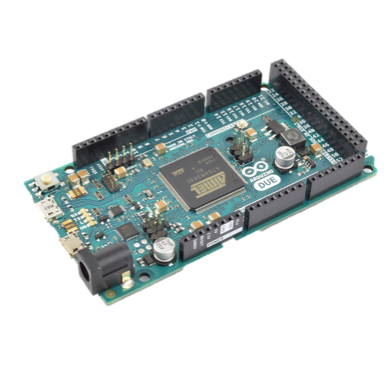
\includegraphics[width=\textwidth]{figures/step1_figureA.png}
    \end{subfigure}
\end{figure}

\pause 

\begin{itemize}
\item 
use of counter\-example guided inductive synthesis (CEGIS)\\ 
to automate design of sound digital controllers 
\end{itemize} 

\end{frame}

\begin{frame}[fragile]{CPS Setup: Continuous Plant and Digital Controller}

\begin{figure}[htb]
\centering

\tikzset{add/.style n args={4}{
    minimum width=6mm,
    path picture={
        \draw[circle] 
            (path picture bounding box.south east) -- (path picture bounding box.north west)
            (path picture bounding box.south west) -- (path picture bounding box.north east);
        \node[draw=none] at ($(path picture bounding box.south)+(0,0.13)$)     {\small #1};
        \node[draw=none] at ($(path picture bounding box.west)+(0.13,0)$)      {\small #2};
        \node[draw=none] at ($(path picture bounding box.north)+(0,-0.13)$)    {\small #3};
        \node[draw=none] at ($(path picture bounding box.east)+(-0.13,0)$)     {\small #4};
        }
    }
 }

\resizebox{1.0\textwidth}{!}{
 \begin{tikzpicture}[scale=0.6,-,>=stealth',shorten >=.2pt,auto,
     semithick, initial text=, ampersand replacement=\&,]

  \matrix[nodes={draw, fill=none, shape=rectangle, minimum height=.2cm, minimum width=.2cm, align=center}, row sep=.6cm, column sep=.2cm] {
    \node[draw=none] (r) {$R(z)$};
%   \& \coordinate (aux0);
   \& \node[circle,add={-}{+}{}{}] (circle) {};
   \node[draw=none] (ez) at ([xshift=.9cm,yshift=.2cm]circle)  {$e(z)$};
   \& \node[rectangle,draw,
	minimum width=1cm,
	minimum height=1cm,
        label=\textbf{Controller}] (cz) at ([xshift=.5cm,yshift=0cm]circle) {\sc $\hat{C}(z)$};
   \node[draw=none] (ud) at ([xshift=1cm,yshift=.2cm]cz)  {$U(z)$};
 
 \only<1>{
 \& \node[rectangle,draw,minimum width=3cm,
	minimum height=1.6cm,] (bbdac) {\sc DAC};
 }
 \only<2->{
   \& complexnode/.pic={ 
      \node[rectangle,draw,
	minimum width=4cm,
	minimum height=1.6cm,
	label=\textbf{DAC},] (dac) {};
     \node[circle,add={}{+}{+}{},fill=gray!20] (q2) at ([xshift=-.65cm]dac.center) {};
     \node[draw=none] (q2t)  at ([xshift=-.65cm,yshift=-.65cm]dac.center) {{\sc Q2}};
     \node[draw=none] (v2)  at ([xshift=-.65cm,yshift=1.5cm]dac.center) {$\nu_2(z)$};
     \node[fill=gray!20] (zoh) at ([xshift=.65cm]dac.center) {{\sc ZOH}};} 
     }
   \& \node[rectangle,draw,
	minimum width=1cm,
	minimum height=1cm,
        label=\textbf{Plant}] (gs) {{\sc $\hat{G}(s)$}};
   \node[draw=none] (ud) at ([xshift=-1cm,yshift=.2cm]gs)  {$U(s)$};
   \node[draw=none] (y) at ([xshift=1cm,yshift=.2cm]gs)  {$\hat{Y}(s)$};
 \only<1>{
 \& \node[rectangle,draw,minimum width=4cm,
	minimum height=1.6cm,] (bbadc) {\sc ADC};
 }   
 \only<2->{
   \& complexnode/.pic={ 
     \node[rectangle,draw,
	minimum width=4cm,
	minimum height=1.6cm,
	label=\textbf{ADC},] (adc) {};
   \draw[] ([xshift=-1cm]adc.center) -- ++(0.5,0.2cm);
   \coordinate (switch1) at ([xshift=-1cm]adc.center);
   \coordinate (switch2) at ([xshift=-0.4cm]adc.center);
   \node[circle,add={}{+}{+}{},fill=gray!20] (q1) at ([xshift=1cm]adc.center) {};} 
     \node[draw=none] (q2t)  at ([xshift=1cm,yshift=-.65cm]adc.center) {{\sc Q1}};
   \node[draw=none] (v1)  at ([xshift=1cm,yshift=1.5cm]adc.center) {$\nu_1(z)$};
   }
   \& \coordinate (aux1);
   \& \node[draw=none] (yz) {$\hat {Y}(z)$};\\
   \& \coordinate (aux3);
   \&
   \&
   \& 
   \& 
   \& \coordinate (aux2);\\
  };


  \path[->] (r) edge (circle.west);
  \path[->] (aux1) edge (yz);
  \path (circle.east) edge (cz);
  \only<1> {
   \path
     (cz.east) edge (bbdac.west)
     (bbdac.east) edge (gs.west);
   \path
      (gs.east) edge (bbadc.west)
      (bbadc.east) edge (aux1.west);
  }
   \only<2->{
  \path[->] (v2) edge (q2.north);
  \path  
   (cz.east) edge (q2.west)
   (q2.east) edge (zoh.west)
   (zoh.east) edge (gs.west);
  \path[->] (v1) edge (q1.north);
  \path
   (gs.east) edge (switch1.west)
   (switch2) edge (q1.west)
   (q1.east) edge (aux1.west);
  }
  \path
   (aux1.south) edge (aux2.north)
   (aux2.west) edge (aux3.east); 
  \path[->]  (aux3.north) edge (circle.south);
 \end{tikzpicture}
}
% \caption{Closed-loop digital control system \label{fig:sampledsystem}}
\end{figure}

%\end{frame}

%\begin{frame}[fragile]{Discrete Time Model}

\uncover<3->
{
\begin{figure}[ht]
\centering
\tikzset{add/.style n args={4}{
    minimum width=6mm,
    path picture={
        \draw[circle] 
            (path picture bounding box.south east) -- (path picture bounding box.north west)
            (path picture bounding box.south west) -- (path picture bounding box.north east);
        \node[draw=none] at ($(path picture bounding box.south)+(0,0.13)$)     {\small #1};
        \node[draw=none] at ($(path picture bounding box.west)+(0.13,0)$)      {\small #2};
        \node[draw=none] at ($(path picture bounding box.north)+(0,-0.13)$)    {\small #3};
        \node[draw=none] at ($(path picture bounding box.east)+(-0.13,0)$)     {\small #4};
        }
    }
 }

\resizebox{1.0\textwidth}{!}{
 \begin{tikzpicture}[scale=0.3,-,>=stealth',shorten >=.2pt,auto,
     semithick, initial text=, ampersand replacement=\&,]

  \matrix[nodes={draw, fill=none, shape=rectangle, minimum height=.2cm, minimum width=.2cm, align=center}, row sep=.6cm, column sep=.3cm] {
    \node[draw=none] (r) {$R(z)$};
%   \& \coordinate (aux0);
   \& \node[circle,add={-}{+}{}{}] (circle) {};
   \node[draw=none] (ez) at ([xshift=1cm,yshift=.15cm]circle)  {$e(z)$};
   \& \node[rectangle,draw,
	minimum width=1cm,
	minimum height=1cm,
        label=\textbf{Controller}] (cz) {\sc $\hat{C}(z)$};
   \node[draw=none] (ud) at ([xshift=1cm,yshift=.15cm]cz)  {$U(z)$};
   \& \node[circle,add={}{+}{+}{}] (circle2) {};
   \node[draw=none] (nu2) at ([yshift=1cm]circle2)  {$\nu_2(z)$};
   \& \node[rectangle,draw,
	minimum width=1cm,
	minimum height=1cm,
        label=\textbf{Plant}] (gs) {{\sc $\hat{G}(z)$}};

   \& \node[circle,add={}{+}{+}{}] (circle3) {};
   \node[draw=none] (nu1) at ([yshift=1cm]circle3)  {$\nu_1(z)$};
   \& \coordinate (aux1);
   \& \node[draw=none] (yz) {$\hat Y(z)$};\\
   \& \coordinate (aux3); 
   \&
   \& 
   \& 
   \&
   \& \coordinate (aux2);\\
  };

  \path[->] (r) edge (circle.west);
  \path[->] (nu2) edge (circle2.north);
  \path[->] (nu1) edge (circle3.north);
  \path[->] (aux1) edge (yz);
  \path  
   (circle.east) edge (cz)
   (cz.east) edge (circle2.west)
   (circle2.east) edge (gs.west)
   (gs.east) edge (circle3.west)
   (circle3.east) edge (aux1.west)
   (aux1.south) edge (aux2.north)
   (aux2.west) edge (aux3.east); 
  \path[->]  (aux3.north) edge (circle.south);
 \end{tikzpicture}
}
%\caption{Fully digital equivalent to system in Figure~\ref{fig:sampledsystem} 
%\label{fig:digsystem1}}
\end{figure}
}

\only<4>{
\begin{displaymath}
\hat{G}(z) = (1-z^{-1})\mathcal{Z}\left\lbrace{\mathcal{L}^{-1}\left\lbrace{\frac{\hat{G}(s)}{s}}\right\rbrace_{t=kT}}\right\rbrace
\end{displaymath}
}

%\only<2-3>{
%\begin{displaymath}
%\hat{Y}(z)=\nu_{1}(z)+\hat{G}(z)\hat{C}(z)R(z)+\hat{G}(z)\nu_{2}(z)-\hat{G}(z)\hat{C}(z)\hat{Y}(z)
%\end{displaymath}
%}

\only<5>{
\begin{equation*}
\hat{Y}(z) = 
\frac{\hat{G}(z) \hat{C}(z)}{1+\hat{G}(z) \hat{C}(z)}R(z) + 
\frac{1}{1+\hat{G}(z) \hat{C}(z)} \nu_{1}(z) + 
\frac{\hat{G}(z)}{1+\hat{G}(z) \hat{C}(z)} \nu_{2}(z) 
\end{equation*}
}

\uncover<6>{
Common denominator:
$$\hat{G}_n(z) \hat{C}_n(z)+\hat{G}_d(z) \hat{C}_d(z)$$ 
}

\end{frame}

\begin{frame}{Stability Analysis via Jury's Criterion}

\begin{equation*}
S(z) = \hat{G}_n(z) \hat{C}_n(z)+\hat{G}_d(z) \hat{C}_d(z) = \sum_{i=0}^{N_S} c_iz^{N_s-i}, c_0 \neq 0 
\end{equation*}

$$
M=\left( 
\begin{array}{ccc}
v^{(0)}_{1} &\cdots & v^{(0)}_{N_S}\\
v^{(1)}_{1} &\cdots&  v^{(1)}_{N_S}\\
\vdots&\vdots&\vdots\\
v^{(N_S-1)}_{1} &\cdots&  v^{(N_S-1)}_{N_S}\\
\end{array}
\right), $$
%
$$
v_{j}^{(k)}=\left\{
\begin{array}{ll}
c_{j-1}, & k=0\\
0,&k>0 \wedge \mbox{if}~j>N_S-k\\
v_{1}^{(k-1)}-v_{N_S-j}^{(k-1)} . \frac{v_{1}^{(k-1)}}{v_{N_S-k}^{(k-1)}}, &k>0 \wedge  \mbox{if}~j\leq N_S-k\\
\end{array}
\right.
$$
%
\begin{eqnarray*}
&S(z) \text{ is stable } \Leftrightarrow& \\ 
%\phi_\mathit{stability} \equiv 
&\textcolor{blue}{S(1) > 0}\ \uncover<2->{\wedge\ \textcolor{blue}{(-1)^{N_S} S(-1) > 0}}\ \uncover<3->{\wedge\ \textcolor{blue}{|c_0| < c_{N_S}}}\ \uncover<4>{\wedge\ \textcolor{blue}{\forall k, v_1^{(k)} > 0}}&
\end{eqnarray*}

\end{frame}

\begin{frame}{Transfer Functions and Uncertainty}

\begin{align*}
\small
\hat{C}(z)&=\frac{\hat{C}_n(z)}{\hat{C}_d(z)}=\frac{\sum_{i=0}^{M_C}(\beta_{i}+\Delta\beta_{i}) z^{-i}}{\sum_{i=0}^{N_C}(\alpha_{i}+\Delta \alpha_{i}) z^{-i}}, \\
\\%\label{plant_tf}
\hat{G}(z)&=\frac{\hat{G}_n(z)}{\hat{G}_d(z)}=\frac{\sum_{i=0}^{M_G}(b_{i}+\Delta b_i) z^{-i}}{\sum_{i=0}^{N_G}(a_{i}+\Delta a_{i}) z^{-i}}.
\end{align*}
%
\begin{itemize}
\item 
$\vec{\beta}$ and $\vec{\alpha}$ -- vectors containing controller coefficients 
\item 
$\vec{b}$ and $\vec{a}$ -- plant coefficients 
\end{itemize}

\end{frame}

\begin{frame}{Sources of Uncertainty}
\setbeamertemplate{itemize items}[square]

\begin{itemize}
\item<1->[1.] Model Parametric Errors (affect $\Delta G(z)$)
\item<2->[2.] Quantisation errors in the ADC, DAC, and controller arithmetics  
(modelled as external noise, do not affect transfer functions)
\item<3->[3.] Roundoff errors in verification process (affect $\Delta S(z)$)
\item<4->[4.] Discretisation errors (affect $\Delta G(z)$ and $\Delta C(z)$) 
\end{itemize}
\end{frame}

\begin{frame}[fragile]{Pole Placement}

\pgfplotsset{grid style={dotted,gray}}
\pgfplotsset{minor grid style={dotted,gray}}
\pgfplotsset{major grid style={dotted,gray}}

\begin{figure}
\centering
\begin{tikzpicture}[scale=1]
\begin{axis}[xmin=-2.5,xmax=2.5,ymin=-2,ymax=2]
\draw[dashed,color=red] (axis cs:0cm,0cm) circle[radius=100];
\node at (axis cs:.5,-.866) [pin={-80:{stable region}},inner sep=0pt] {};
\draw[color=blue] (axis cs:0.5,0.7) ellipse[x radius=5, y radius=15];
\node at (axis cs:.5,.7) [pin={+10:poles},inner sep=0pt] {};
\end{axis}
\end{tikzpicture}
\end{figure}
\end{frame}


%\begin{frame}[fragile]
%\begin{figure}
%\centering
%\begin{tikzpicture}[scale=1]
%\begin{axis}[xmin=-2.5,xmax=2.5,ymin=-2,ymax=2, minor xtick={-2,-1.75, ..., 2}, minor ytick={-2,-1.75, ..., 2}, grid=both]
%\draw[dashed,color=red] (axis cs:0cm,0cm) circle[radius=100];
%\node at (axis cs:.7,-.7) [pin={-10:stable},inner sep=0pt] {};
%\only<1>{
%\draw[color=blue] (axis cs:0.5,0.7)  ellipse[x radius=5, y radius=15];
%\node at (axis cs:.5,.7) [pin={+10:poles},inner sep=0pt] {};
%}
%\only<2>{
%\draw[color=orange] (axis cs:0.5,0.75) ellipse[x radius=5, y radius=15];
%\node at (axis cs:.5,.75) [pin={+10:poles},inner sep=0pt] {};
%}
%\end{axis}
%\end{tikzpicture}
%\end{figure}
%\end{frame}

\begin{frame}[fragile]{Pole Placement}
\begin{figure}
\centering
\begin{tikzpicture}[scale=1]
\begin{axis}[xmin=0,xmax=1.5,ymin=0,ymax=1]
\draw[dashed,color=red] (axis cs:0cm,0cm) circle[radius=100];
\node at (axis cs:.7,-.7) [pin={-10:stable},inner sep=0pt] {};
\draw[color=blue] (axis cs:0.5,0.7) ellipse[x radius=5, y radius=15];
\node at (axis cs:.5,.7) [pin={+10:poles},inner sep=0pt] {};
\end{axis}
\end{tikzpicture}
\end{figure}
\end{frame}

\begin{frame}[fragile]{Pole Placement in a Discretized Domain}

\pgfplotsset{grid style={dotted,gray}}
\pgfplotsset{minor grid style={dotted,gray}}
\pgfplotsset{major grid style={dotted,gray}}

\begin{figure}
\centering
\begin{tikzpicture}[scale=1]
\begin{axis}[xmin=0,xmax=1.25,ymin=0,ymax=1, xtick={0,0.25, ..., 1.25}, ytick={0,0.25, ..., 1.25}, grid=both]
\draw[dashed,color=red] (axis cs:0cm,0cm) circle[radius=100];
\node at (axis cs:.7,-.7) [pin={-10:stable},inner sep=0pt] {};
\only<1>{
\draw[color=blue] (axis cs:0.5,0.7)  ellipse[x radius=5, y radius=15];
\node at (axis cs:.5,.7) [pin={+10:poles},inner sep=0pt] {};
}
\only<2>{
\draw[color=orange] (axis cs:0.5,0.75) ellipse[x radius=5, y radius=15];
\node at (axis cs:.5,.75) [pin={+10:poles},inner sep=0pt] {};
}
\end{axis}
\end{tikzpicture}
\end{figure}
\end{frame}

%
\begin{frame}{Objective}

We seek to synthesise a controller where $\Delta \vec{\beta}=0$ and $\Delta \vec{\alpha}=0$ and which stabilizes all plants within a given range of $\Delta \vec{b}$ and $\Delta \vec{a}$. 

\begin{figure}[htb]
\centering
\resizebox{1.0\textwidth}{!}
{
 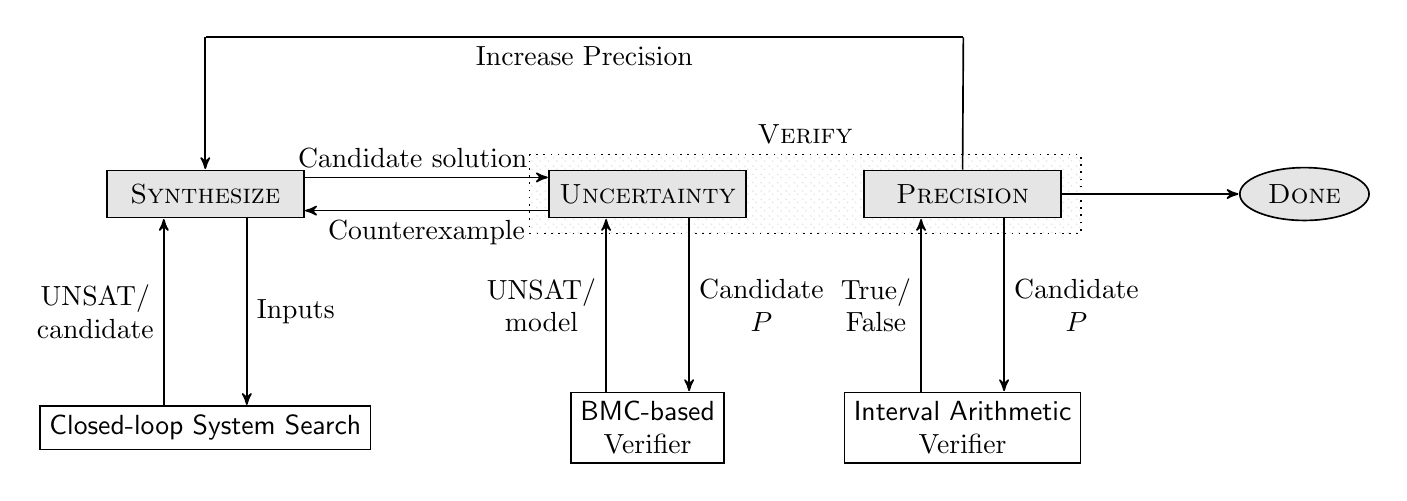
\begin{tikzpicture}[scale=0.3,->,>=stealth',shorten >=.2pt,auto, semithick, initial text=, ampersand replacement=\&,]
  \matrix[nodes={draw, fill=none, shape=rectangle, minimum height=.2cm, minimum width=.2cm, align=center
},
          row sep=1cm, column sep=2cm] {
   \coordinate (aux1);
   \& \coordinate (aux2);
   \&;\\
   \node[minimum width=2.5cm, minimum height=0.6cm, fill=gray!20] (synth) {{\sc Synthesize}};
   \&
   complexnode/.pic={ 
     \node[rectangle,draw,dotted,
	minimum width=7cm,
	minimum height=1cm,
        pattern=north west lines, pattern color=gray!20,
	label={\sc Verify},] (verif) {};
     \node[minimum width=2.5cm, minimum height=0.6cm, fill=gray!20] (verif1) at ([xshift=-2cm]verif.center) {{\sc Uncertainty}};
     \node[minimum width=2.5cm, minimum height=0.6cm, fill=gray!20] (verif2) at ([xshift=2cm]verif.center) {{\sc Precision}};
   } 
   \& \node[ellipse, fill=gray!20] (done) {{\sc Done}};\\
   \& \\
   \node[minimum height=0.5cm] (gp) {\sf Closed-loop System Search};
   \&
   complexnode/.pic={ 
     \coordinate (aux);
   \node[minimum height=0.5cm] (bmc) at ([xshift=-2cm]aux.center) {\sf BMC-based\\Verifier};
   \node[minimum height=0.5cm] (fp)  at ([xshift=2cm]aux.center) {\sf Interval Arithmetic\\Verifier};
   }   
    \\
  };

   \path (verif2) edge node {} (done);
   \path ([xshift=5em]synth.south) edge node[align=center] {Inputs} ([xshift=5em]gp.north);
   \path ([xshift=-5em]gp.north) edge node[align=center] {UNSAT/\\candidate} ([xshift=-5em]synth.south);
   \path ([yshift=2em]synth.east) edge node[xshift=-0.5em] {Candidate solution} ([yshift=2em]verif1.west);
   \path  ([xshift=5em]verif1.south) edge node[align=center] {Candidate\\ $P$} ([xshift=5em]bmc.north);
   \path  ([xshift=-5em]bmc.north) edge node[align=center]  {UNSAT/\\model} ([xshift=-5em]verif1.south);
   \path ([yshift=-2em]verif1.west) edge node {Counterexample} ([yshift=-2em]synth.east);
   \path ([xshift=5em]verif2.south) edge node[align=center] {Candidate\\ $P$} ([xshift=5em]fp.north);
   \path  ([xshift=-5em]fp.north) edge node[align=center]  {True/\\False} ([xshift=-5em]verif2.south);
   \path (aux1) edge (synth.north);
   \path[-] (verif2.north) edge node[align=center] {} ([xshift=6.7cm]aux2);
   \path[-] ([xshift=6.7cm]aux2) edge node[align=center] {Increase Precision} (aux1);
 \end{tikzpicture}
}
\end{figure}

\end{frame}

\begin{frame}{Case Study}

Take a classical cruise control example from the literature. 
%
\begin{equation*}
G(z) = \frac{0.0264}{z-0.9998}.
\end{equation*}

Using an optimization tool, the following stable high-performance
controller was designed:
%
\begin{equation*}
C(z) = \frac{2.72z^2 - 4.153z + 1.896}{z^2 - 1.844z + 0.8496}.
\end{equation*}
%
However, if we implement the controller in $\mathbb{R} \langle 4,16\rangle$.
%
\begin{equation*}
\resizebox{.9\textwidth}{!}{
$\tilde{C}(z) {:=} \frac{2.7199859619140625z^2{-}4.1529998779296875z
{+}1.89599609375}{z^2{-}1.843994140625z+0.8495941162109375}$. 
}
\end{equation*} 
%
where $\tilde{C}(z)$ is the controller adjusted to the FWL. The resulting system is unstable. 

\end{frame}

\begin{frame}[fragile]{CEGIS Architecture}
\begin{figure}[htb]
\centering
\resizebox{1.0\textwidth}{!}
{
 \begin{tikzpicture}[scale=0.3,->,>=stealth',shorten >=.2pt,auto, semithick, initial text=, ampersand replacement=\&,]
  \matrix[nodes={draw, fill=none, shape=rectangle, minimum height=.2cm, minimum width=.2cm, align=center
},
          row sep=1cm, column sep=2cm] {
   \coordinate (aux1);
   \& \coordinate (aux2);
   \&;\\
   \node[minimum width=2.5cm, minimum height=0.6cm, fill=gray!20] (synth) {{\sc Synthesize}};
   \&
   complexnode/.pic={ 
     \node[rectangle,draw,dotted,
	minimum width=7cm,
	minimum height=1cm,
        pattern=north west lines, pattern color=gray!20,
	label={\sc Verify},] (verif) {};
     \node[minimum width=2.5cm, minimum height=0.6cm, fill=gray!20] (verif1) at ([xshift=-2cm]verif.center) {{\sc Uncertainty}};
     \node[minimum width=2.5cm, minimum height=0.6cm, fill=gray!20] (verif2) at ([xshift=2cm]verif.center) {{\sc Precision}};
   } 
   \only<1,22>{\& \node[ellipse, fill=gray!20] (done) {{\sc Done}};}\\
   \& \\
   \node[minimum height=0.5cm] (gp) {\sf Closed-loop System Search\\ \only<2-15>{$\textcolor{blue}{FP=\mathbb{R}\langle16,24\rangle}$}\only<16->{$\textcolor{blue}{FP=\mathbb{R}\langle20,28\rangle}$}};
   \&
   complexnode/.pic={ 
     \coordinate (aux);
   \node[minimum height=0.5cm] (bmc) at ([xshift=-2cm]aux.center) {\sf BMC-based\\Verifier};
   \node[minimum height=0.5cm] (fp)  at ([xshift=2cm]aux.center) {\sf Interval Arithmetic\\Verifier};
   }   
    \\
  };

   \only<1,22>{\path (verif2) edge node {} (done);}
   \only<1>{\path ([xshift=5em]synth.south) edge node[align=center] {Inputs} ([xshift=5em]gp.north);}
   \only<2-7,16-17>{\path ([xshift=5em]synth.south) edge node[align=center] {$\textcolor{blue}{\frac{0.0264}{z-0.9998}}$} ([xshift=5em]gp.north);}
   \only<1-2,8,16,18>{\path ([xshift=-5em]gp.north) edge node[align=center] {UNSAT/\\candidate} ([xshift=-5em]synth.south);}
   \only<3-7,17>{\path ([xshift=-5em]gp.north) edge node[align=center] {$\textcolor{blue}{\frac{0z^2+0z+0}{0z^2+0z+0}}$} ([xshift=-5em]synth.south);}
   \only<1-3,8-9,16,18>{\path ([yshift=2em]synth.east) edge node[xshift=-0.5em] {Candidate solution} ([yshift=2em]verif1.west);}
   \only<4-7,17>{\path ([yshift=2em]synth.east) edge node[xshift=-0.5em] {$\textcolor{blue}{\frac{0z^2+0z+0}{0z^2+0z+0}}$} ([yshift=2em]verif1.west);}
   \only<1-4,8-10,16,18-19>{\path  ([xshift=5em]verif1.south) edge node[align=center] {Candidate\\ $P$} ([xshift=5em]bmc.north);}
   \only<5-7,17>{\path  ([xshift=5em]verif1.south) edge node[align=center] {$\textcolor{blue}{\frac{0z^2+0z+0}{0z^2+0z+0}}$} ([xshift=5em]bmc.north);}
   \only<1-5,8-11,16,18-19>{\path  ([xshift=-5em]bmc.north) edge node[align=center]  {UNSAT/\\model} ([xshift=-5em]verif1.south);}
   \only<6-7>{\path  ([xshift=-5em]bmc.north) edge node[align=center]  {$\textcolor{blue}{\frac{0.026506}{1.000610z+1.002838}}$} ([xshift=-5em]verif1.south);}
   \only<1-6,8-16,18->{\path ([yshift=-2em]verif1.west) edge node {Counterexample} ([yshift=-2em]synth.east);}
   \only<7>{\path ([yshift=-2em]verif1.west) edge node {$\textcolor{blue}{\frac{0.026506}{1.000610z+1.002838}}$} ([yshift=-2em]synth.east);}
   \only<8-15>{\path ([xshift=5em]synth.south) edge node[align=center] {$\textcolor{blue}{\frac{0.0264}{z-0.9998}}$\\$\textcolor{blue}{\frac{0.026506}{1.000610z+1.002838}}$} ([xshift=5em]gp.north);}
   \only<9-15,19->{\path ([xshift=-5em]gp.north) edge node[align=center] {$\textcolor{blue}{\hat{C}(z)}$} ([xshift=-5em]synth.south);}
   \only<10-15>{\path ([yshift=2em]synth.east) edge node[xshift=-0.5em] {$\textcolor{blue}{\frac{12.402664z^2{-}11.439667z{+}0.596756}{4.003906z^2{-}0.287949z{+}0.015625}}$} ([yshift=2em]verif1.west);}
   \only<11-15,20->{\path  ([xshift=5em]verif1.south) edge node[align=center] {$\textcolor{blue}{\hat{C}(z)}$} ([xshift=5em]bmc.north);}
   \only<12-15,20->{\path  ([xshift=-5em]bmc.north) edge node[align=center]  {\textcolor{blue}{UNSAT}\\\textcolor{blue}{Pass}} ([xshift=-5em]verif1.south);}
   \only<1-12,16-20>{\path ([xshift=5em]verif2.south) edge node[align=center] {Candidate\\ $P$} ([xshift=5em]fp.north);}
   \only<13-15,21->{\path ([xshift=5em]verif2.south) edge node[align=center] {$\textcolor{blue}{\hat{C}(z)}$} ([xshift=5em]fp.north);}
   \only<1-13,16-20>{\path  ([xshift=-5em]fp.north) edge node[align=center]  {True/\\False} ([xshift=-5em]verif2.south);}
   \only<14-15>{\path  ([xshift=-5em]fp.north) edge node[align=center]  {\textcolor{blue}{False}} ([xshift=-5em]verif2.south);}
   %\only<15>{\path ([yshift=-2em]verif1.west) edge node {\textcolor{blue}{precision}} ([yshift=-2em]synth.east);}
   \only<17>{\path  ([xshift=-5em]bmc.north) edge node[align=center]  {$\textcolor{blue}{\frac{0.026314}{0.999024z{-}1.004785}}$} ([xshift=-5em]verif1.south);}
   \only<17>{\path ([yshift=-2em]verif1.west) edge node {$\textcolor{blue}{\frac{0.026314}{0.999024z{-}1.004785}}$} ([yshift=-2em]synth.east);}
   \only<18->{\path ([xshift=5em]synth.south) edge node[align=center] {$\textcolor{blue}{\frac{0.0264}{z-0.9998}}$\\$\textcolor{blue}{\frac{0.026314}{0.999024z{-}1.004785}}$} ([xshift=5em]gp.north);}
   \only<19->{\path ([yshift=2em]synth.east) edge node[xshift=-0.5em] {$\textcolor{blue}{\frac{11.035202z^2{+}5.846100z{+}4.901855}{1.097901z^2{+}0.063110z{+}0.128357}}$} ([yshift=2em]verif1.west);}
   \only<21->{\path  ([xshift=-5em]fp.north) edge node[align=center]  {\textcolor{blue}{True}} ([xshift=-5em]verif2.south);}




   \path (aux1) edge (synth.north);
   \path[-] (verif2.north) edge node[align=center] {} ([xshift=6.7cm]aux2);
   \only<1-14,16-> {\path[-] ([xshift=6.7cm]aux2) edge node[align=center] {Increase Precision} (aux1);}
   \only<15> {\path[-] ([xshift=6.7cm]aux2) edge node[align=center] {\textcolor{blue}{Increase Precision}} (aux1);}
 \end{tikzpicture}
}
\end{figure}
\end{frame}

%\begin{frame}
%
%\begin{itemize*}
%
%\item We automatically generate {\em correct-by-construction} digital
%  controllers using an inductive synthesis approach.  Our application of program
%  synthesis is non-trivial and addresses challenges specific to control
%  systems, such as quantizers and FWL.  In particular, we
%  have found that a two-stage verification engine that continuously refines
%  the precision of the fixed-point representation of the plant yields a
%  speed-up of two orders of magnitude over a conventional one-stage
%  verification engine.
%
%\item Experimental results show that \tool is able to efficiently synthesize
%  stable controllers for a set of intricate benchmarks taken from the
%  literature: the median runtime for our benchmark set considering the
%  faster engine is $48$\,s, i.e., half of the controllers can be synthesized
%  in less than one minute.
%
%\end{itemize*}
%\end{frame}

%
%
%%%%%%%%%%%%%%%%%%%%%%%%%%%%%%%%%%%%%%%%%%%%%%%%%%%%%%%%%%%%%%%%%%%%%%%%%%%%%%%%%%%%%%%
%\subsection{Illustrative Example} \label{sec:running-ex}
%
%We illustrate our approach with a classical cruise control example from the
%literature~\cite{Astrom08}.  It highlights the challenges that
%arise when using finite-precision arithmetic in digital control.  We are
%given a discrete plant model (with a time step of $0.2$\,s), 
%represented by the following $z$-expression:
%%
%\begin{equation}
%\label{Eq:running-example-plant}
%G(z) = \frac{0.0264}{z-0.9998}.
%\end{equation}
%
%Using an optimization tool, the authors
%of~\cite{DBLP:conf/hybrid/WangGRJF16} have designed a high-performance
%controller for this plant, which is characterized by the following
%$z$-domain transfer function:
%%
%\begin{equation}
%\label{Eq:running-example-controller}
%C(z) = \frac{2.72z^2 - 4.153z + 1.896}{z^2 - 1.844z + 0.8496}.
%\end{equation}
%%
%The authors of~\cite{DBLP:conf/hybrid/WangGRJF16} claim that the controller
%$C(z)$ in~\eqref{Eq:running-example-controller} stabilizes the closed-loop
%system for the discrete plant model $G(z)$
%in~\eqref{Eq:running-example-plant}.  However, if the effects of
%finite-precision arithmetic are considered, then this closed-loop system
%becomes unstable.
%%
%For instance, an implementation of $C(z)$ using 
%$\mathbb R \param {4}{16}$ fixed-point
%numbers (i.e., $4$ bits for the integer part and $16$ bits for the
%fractional part) can be modeled as: 
%%
%\begin{equation}
%\label{Eq:running-example-controller-quantized}
%\resizebox{.47\textwidth}{!}{
%$\tilde{C}(z) {:=} \frac{2.7199859619140625z^2{-}4.1529998779296875z
%{+}1.89599609375}{z^2{-}1.843994140625z+0.8495941162109375}$. 
%}
%\end{equation} 
%%
%The resulting system, 
%%using the typical series loop configuration, 
%where $\tilde{C}(z)$ and $G(z)$ are in the forward path, is unstable. 
%Notice that this is disregarding further approximation effects on the plant caused by quantization in the verifier (i.e., $\tilde{G}(z)$).
%%\aabatecmt{[hang in there - did we not consider FWL on $G(z)$? why not?]}
%%\dariocmt{we are explaining the case where a real plant (no FWL) is not correctly stabilized by $\tilde{C}$, so although our analysis might evaluate $\tilde{G}(z)$, the problem statement is over $G(z)$}
%Figure~\ref{fig:original} gives the Bode diagram for the digital controller
%represented in~\eqref{Eq:running-example-controller}: 
%as the phase margin is negative, 
%the controller is unstable when considering the FWL effects.

\begin{frame}[fragile]{Outcomes: Step Response}
\begin{figure}
    \centering
    \begin{subfigure}[b]{0.3\textwidth}
        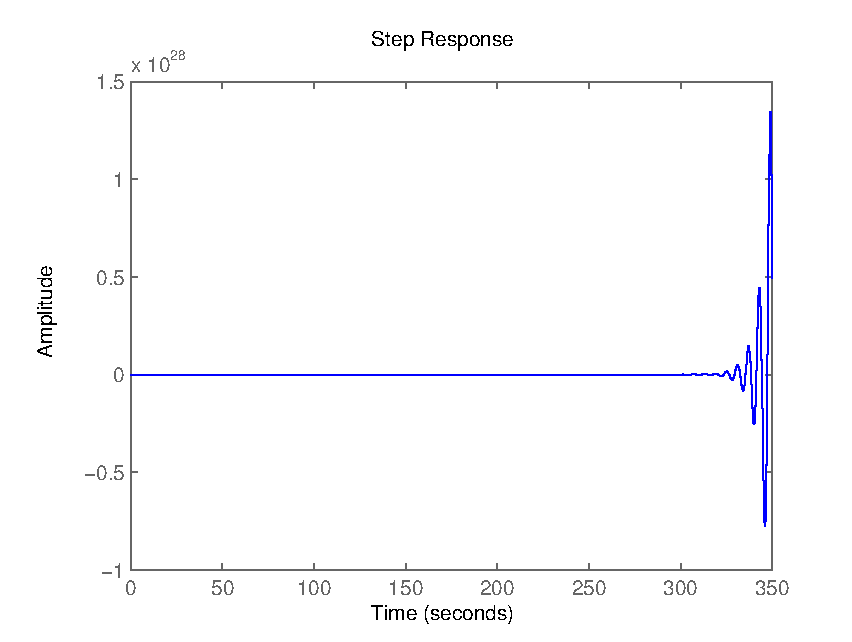
\includegraphics[width=\textwidth]{figures/runningexample_step0.pdf}
        \caption{Original\\ controller}
        \label{fig:step0}
    \end{subfigure}
    ~
    \begin{subfigure}[b]{0.3\textwidth}
        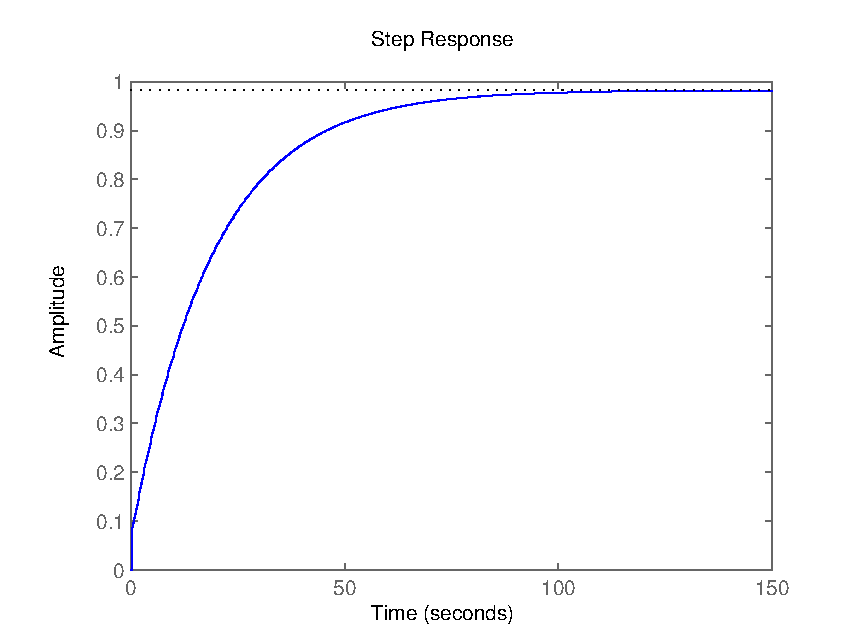
\includegraphics[width=\textwidth]{figures/runningexample_step1.pdf}
        \caption{Controller (first step)}
        \label{fig:step1}
    \end{subfigure}
    ~
    \begin{subfigure}[b]{0.3\textwidth}
        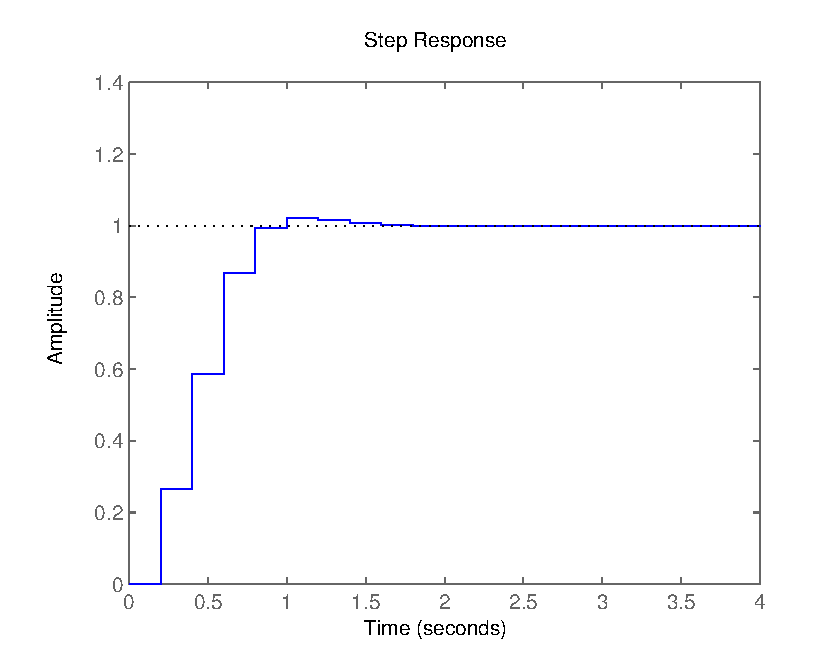
\includegraphics[width=\textwidth]{figures/runningexample_step2.pdf}
        \caption{Controller (final step)}
        \label{fig:step2}
    \end{subfigure}
\end{figure}

\begin{itemize} 
\item 
original controller was synthesised ignoring FWL effects (becomes unstable over time) 
\end{itemize}

\end{frame}


\begin{frame}[fragile]{Outcomes: Controller Order}
\begin{figure}
 \begin{tikzpicture}
\begin{axis}[ylabel=order,xlabel=time,xmode=log
]
\addplot[scatter,only marks,mark=*] table{./results.dat};
\end{axis}
\end{tikzpicture}
\end{figure}
\end{frame}

\begin{frame}[fragile]{Outcomes: Benchmark}

\begin{table}
\centering
\scalebox{0.6}{
\begin{tabular}{| r | c | l | r r || r | r |}
\hline
\# & Plant  & Benchmark                  & $I$ & $F$
   & 2-stage & 1-stage
    \\\hline\hline
1  & $G_{1a}$  & CruiseControl02
            &   4 &  16 & \textbf{12\,s}   & 67\,s     \\
2  & $G_{1b}$  & CruiseControl02$^\dagger$
            &   4 &  16 & 14600\,s   & \textbf{52\,s}     \\
3  & $G_{2a}$  & SpgMsDamper
            &  15 &  16 & \textbf{52\,s}   & 318\,s     \\
4  & $G_{2b}$  & SpgMsDamper$^\dagger$
            &  15 &  16 & \xmark  & \xmark    \\
5  & $G_{3a}$  & SatelliteB2
            &   3 &   7 & \textbf{36\,s}    & \xmark     \\
6  & $G_{3b}$  & SatelliteB2$^\dagger$
            &   3 &   7 & \xmark  & \textbf{4111\,s}  \\
7  & $G_{3c}$  & SatelliteC2
            &   3 &   5 & \textbf{3\,s}    & 205\,s    \\
8  & $G_{3d}$  & SatelliteC2$^\dagger$
            &   3 &   5 & \textbf{50\,s}  & 1315\,s    \\
9  & $G_4$  & Cruise
            &   3 &   7 & 1\,s  & 1\,s    \\
10 & $G_5$  & DCMotor
            &   3 &   7 & \textbf{1\,s}  & 10\,s    \\
11 & $G_6$  & DCServomotor
            &   4 &  11 & \textbf{46\,s}  & \xmark    \\
12 & $G_7$  & Doyleetal
            &   4 &  11 & \textbf{8769\,s}  & \xmark    \\
13 & $G_8$  & Helicopter
            &   3 &   7 & \textbf{44\,s}  & \xmark    \\
14 & $G_9$  & Pendulum
            &   3 &   7 & \textbf{1\,s}  & 14826\,s    \\
15 &$G_{10}$& Suspension
            &   3 &   7 & \textbf{1\,s}  & 5\,s    \\
16 &$G_{11}$& Tapedriver
            &   3 &   7 & 1\,s  & 1\,s    \\
17 &$G_{12a}$& a\_ST1\_IMPL1
            &  16 &   4 & \textbf{11748\,s} & \xmark   \\
18 &$G_{12a}$& a\_ST1\_IMPL2
            &  16 &   8 & \textbf{351\,s}  & \xmark   \\
19 &$G_{12a}$& a\_ST1\_IMPL3
            &  16 &  12 & \textbf{8772\,s}   & \xmark   \\
20 &$G_{12b}$& a\_ST2\_IMPL1
            &  16 &   4 & \textbf{1128\,s}  & \xmark   \\
21 &$G_{12b}$& a\_ST2\_IMPL2
            &  16 &   8 & \xmark  & \xmark    \\
22 &$G_{12b}$& a\_ST2\_IMPL3
            &  16 &  12 & \textbf{15183\,s} & \xmark   \\ 
23 &$G_{12c}$& a\_ST3\_IMPL1
            &  16 &   4 & \xmark & \xmark   \\\hline
\end{tabular}}\\[0.2ex]
\caption{\tool results ({\xmark} = time-out, $\dagger$ = 
uncertainty)
\label{tab:results}}
\end{table}
\end{frame} 

\begin{frame}{Conclusions}
\begin{itemize}
\item We have presented a method for automatically synthesizing stable and sound controllers, implemented
in a tool called \tool.
\item \tool marks the first use of the
CEGIS that handles plants with uncertain models and FWL effects over the
digital controller.  
\item Our experimental results show that \tool is able to synthesize
stable controllers for most benchmarks within a reasonable amount of time.  
\item Future work will extend this CEGIS-based
approach to LTI systems with state space safety specifications. 
\end{itemize}
\end{frame}

\begin{frame}[fragile]{LTI Closed Loop System}
\begin{figure}[htb]
\centering

\tikzset{add/.style n args={4}{
    minimum width=6mm,
    path picture={
        \draw[circle] 
            (path picture bounding box.south east) -- (path picture bounding box.north west)
            (path picture bounding box.south west) -- (path picture bounding box.north east);
        \node[draw=none] at ($(path picture bounding box.south)+(0,0.13)$)     {\small #1};
        \node[draw=none] at ($(path picture bounding box.west)+(0.13,0)$)      {\small #2};
        \node[draw=none] at ($(path picture bounding box.north)+(0,-0.13)$)    {\small #3};
        \node[draw=none] at ($(path picture bounding box.east)+(-0.13,0)$)     {\small #4};
        }
    }
 }

\resizebox{1.0\textwidth}{!}{
 \begin{tikzpicture}[scale=0.6,-,>=stealth',shorten >=.2pt,auto,
     semithick, initial text=, ampersand replacement=\&,]

  \matrix[nodes={draw, fill=none, shape=rectangle, minimum height=.2cm, minimum width=.2cm, align=center}, row sep=.6cm, column sep=.6cm] {
    \node[draw=none] (r) {$r_k$};
    
   \& \node[circle,add={-}{+}{\only<3>{+}}{}] (circle) {};
   \only<3>{\node[draw=none] (v12) at ([xshift=0cm,yshift=1cm]circle)  {$\nu_2-\mat{K}_d\nu_1+\nu_3$};}
   \node[draw=none] (ez) at ([xshift=1cm,yshift=.15cm]circle)  {$u_k$};
   \node[rectangle,draw,minimum width=1cm,minimum height=1cm] (Kd) at ([xshift=0,yshift=-1.5cm]circle)  {\sc $\mat{K}_d$};
   \coordinate (kdsouth) at ([yshift=-2cm]Kd);
     
\only<1>{
 \& \node[rectangle,draw,minimum width=3cm,
	minimum height=1.6cm,] (bbdac) {\sc DAC};
 }

\only<2>{   
   \& complexnode/.pic={ 
     \node[rectangle,dashed,draw,minimum width=3cm,minimum height=1.6cm,label=\textbf{DAC}] (dac) {};
     \node[circle,add={+}{+}{}{},fill=gray!20] (q2) at ([xshift=-.65cm]dac.center) {};
     \node[draw=none] (q2t)  at ([yshift=.55cm]q2) {{\sc Q2}};
     \node[draw=none] (v2)  at ([yshift=-1.5cm]q2) {$\nu_2$};
     \node[fill=gray!20] (zoh) at ([xshift=.65cm]dac.center) {\sc ZOH};
   }   
}

   \& complexnode/.pic={ 
      \only<1>{\node[rectangle,dashed,draw,minimum width=6.5cm,minimum height=3.5cm,label=\textbf{Plant}] (plant)  at ([yshift=-.4cm]dac.center) {};}
      \only<2>{\node[rectangle,dashed,draw,minimum width=6.5cm,minimum height=3.5cm,label=\textbf{Plant}] (plant)  at ([yshift=-.5cm]dac.center) {};}
      \only<3>{\node[rectangle,dashed,draw,minimum width=6.5cm,minimum height=3.5cm,label=\textbf{Plant}] (plant)  at ([yshift=-.75cm]dac.center) {};}
      \node[rectangle,draw,minimum width=1cm,minimum height=1cm] (B) at ([xshift=-2cm,yshift=.5cm]plant.center)  {\sc \only<1-2>{$\mat{B}$}\only<3>{$\mat{B}_d$}};
      \node[draw=none] (u) at ([xshift=-.8cm,yshift=.15cm]B)  {\only<1-2>{$u(t)$}};
      \node[circle,add={+}{+}{}{}] (p1) at ([xshift=-0.6cm,yshift=.5cm]plant.center) {};
      \node[draw=none] (xdot) at ([xshift=.9cm,yshift=.2cm]p1)  {\only<1-2>{$\dot{\mat{x}}(t)$}\only<3>{$\mat{x}_{k+1}$}};   
      \node[rectangle,draw,minimum width=1cm] (int) at ([xshift=1.2cm,yshift=.5cm]plant.center) {\sc \only<1-2>{$\int$}\only<3>{$Z^{-1}$}};
      \coordinate (xsouth) at ([xshift=1cm]int);
      \node[draw=none] (x) at ([xshift=1.2cm,yshift=.15cm]int)  {\only<1-2>{$\mat{x}(t)$}\only<3>{$\mat{x}_k$}};
      \node[rectangle,draw,minimum width=1cm,minimum height=1cm] (A) at ([xshift=1.2cm,yshift=-1cm]plant.center)  {\sc \only<1-2>{$\mat{A}$}\only<3>{$\mat{A}_d$}};
      \coordinate (aeast) at ([xshift=1cm]A);
      \coordinate (awest) at ([xshift=-1.8cm]A);
    } 
        
\only<1>{
 \& \node[rectangle,draw,minimum width=3cm,
	minimum height=1.6cm,] (bbadc) {\sc ADC};
     \coordinate (ykeast) at ([xshift=1.9cm]bbadc);
     \coordinate (yksouth) at ([xshift=1.9cm,yshift=-3.5cm]bbadc);
 }
\only<2>{
   \& complexnode/.pic={ 
     \node[rectangle,dashed,draw,minimum width=3.5cm,minimum height=1.6cm,label=\textbf{ADC},] (adc) {};
     \draw[] ([xshift=-1cm]adc.center) -- ++(0.5,0.2cm);
     \coordinate (switch1) at ([xshift=-1cm]adc.center);
     \coordinate (switch2) at ([xshift=-0.4cm]adc.center);
     \node[circle,add={+}{+}{}{},fill=gray!20] (q1) at ([xshift=.6cm]adc.center) {};
     \node[draw=none] (q2t)  at ([yshift=.55cm]q1) {\sc Q1};
     \node[draw=none] (v1)  at ([yshift=-1.5cm]q1) {$\nu_1$};
     \node[draw=none] (y) at ([xshift=.85cm,yshift=.15cm]q1)  {$\mat{x}_k$};} 
     \coordinate (ykeast) at ([xshift=1.9cm]q1);
     \coordinate (yksouth) at ([xshift=1.9cm,yshift=-3.5cm]q1);
   }
   \& \coordinate (aux1);
   \& \\
  };
\only<3>{
   \coordinate (ykeast) at ([xshift=4.5cm]int);
   \coordinate (yksouth) at ([xshift=4.5cm,yshift=-5.8cm]int);
}
  \path[->] (r) edge (circle.west);
  \only<1>{
  \path
    (circle.east) edge (bbdac.west)
    (bbdac.east) edge (B.west);
  }
  \only<2>{
    \path[->] (v2) edge (q2.south);
    \path[->] (circle.east) edge (q2.west);
    \path       (q2.east) edge (zoh.west);
    \path[->] (zoh.east) edge (B.west);
  }
  \only<3>{
    \path[->] (v12) edge (circle.north);
    \path[->] (circle.east) edge (B.west);
  }
  \path
   (B.east) edge (p1.west)
   (p1.east) edge (int.west)
   (xsouth) edge (aeast)
   (aeast) edge (A.east)
   (A.west) edge (awest)
   (awest) edge (p1.south);
   \only<2>{
   \path[->] (v1) edge (q1.south);
   \path   
   (int.east) edge (switch1.west)
   (switch2) edge (q1.west);
   }
\only<1>{ 
  \path 
    (int.east) edge (bbadc.west)
    (bbadc.east) edge (ykeast);
}   
\only<2>{ \path (q1.east) edge (ykeast);}
\only<3>{ \path (int.east) edge (ykeast);}
  \path
   (ykeast) edge (yksouth)
   (yksouth) edge (kdsouth);
  \path[->]  (kdsouth) edge (Kd.south);
  \path (Kd.north) edge (circle.south);
 \end{tikzpicture}
}
\end{figure}
\uncover<3>{
\begin{align*}
A_d &= e^{A T_s} = \mathcal{L}^{-1} { ( s I - A )^{-1} }_{t = T_s}\\
B_d &= \int_{0}^{T_s} e^{A t} dt\ B = A^{-1} ( A_d - I ) B
\end{align*}}
\end{frame}

\begin{frame}[fragile]{Multi-stage Verification CEGIS}
\begin{figure}[htb]
{\scriptsize
\centering
{
 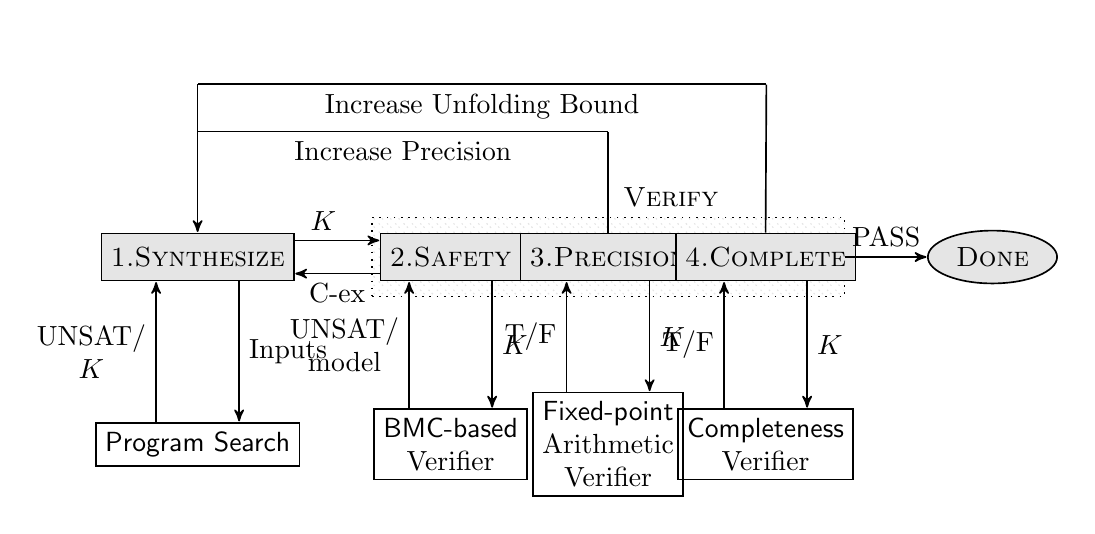
\begin{tikzpicture}[scale=0.3,->,>=stealth',shorten >=.2pt,auto, semithick, initial text=, ampersand replacement=\&,]
  \matrix[nodes={draw, fill=none, shape=rectangle, minimum height=.2cm, minimum width=.2cm, align=center
},
          row sep=.6cm, column sep=.9cm] {
   \coordinate (aux1);
   \& \coordinate (aux2);
   \&;\\
   \coordinate (aux3);
   \& \coordinate (aux4);
   \&;\\
   \coordinate (aux5);
   \& \coordinate (aux6);
   \&;\\
   \node[minimum width=1.5cm, minimum height=0.6cm, fill=gray!20] (synth) {{\sc 1.Synthesize}};
   \&
   complexnode/.pic={ 
     \node[rectangle,draw,dotted,
	minimum width=6cm,
	minimum height=1cm,
        pattern=north west lines, pattern color=gray!20,
	label={\sc ~~~~~~~~~~~~Verify},] (verif) {};
     \node[minimum width=1cm, minimum height=0.6cm, fill=gray!20] (verif1) at ([xshift=-2cm]verif.center) {{\sc 2.Safety}};
     \node[minimum width=1cm, minimum height=0.6cm, fill=gray!20] (verif2) at ([xshift=0cm]verif.center) {{\sc 3.Precision}};
     \node[minimum width=1cm, minimum height=0.6cm, fill=gray!20] (verif3) at ([xshift=2cm]verif.center) {{\sc 4.Complete}};
   } 
   \& \node[ellipse, fill=gray!20] (done) {{\sc Done}};\\
   \& \\
   \node[minimum height=0cm] (gp) {\sf Program Search};
   \&
   complexnode/.pic={ 
     \coordinate (aux);
   \node (bmc) at ([xshift=-2cm]aux.center) {\sf BMC-based \\Verifier};
   \node (fp)  at ([xshift=0cm]aux.center) {\sf Fixed-point \\ Arithmetic\\Verifier};
   \node (sv)  at ([xshift=2cm]aux.center) {\sf Completeness\\Verifier};
   }   
    \\
  };

   \path
    ([yshift=2em]synth.east) edge node[xshift=-0.5em,align=center] {$K$} ([yshift=2em]verif1.west)
    ([yshift=-2em]verif1.west) edge node {C-ex} ([yshift=-2em]synth.east)
    ([xshift=-5em]fp.north) edge node[align=center]  {T/F} ([xshift=-5em]verif2.south)
    ([xshift=-5em]sv.north) edge node[align=center]  {T/F} ([xshift=-5em]verif3.south)
    ([xshift=5em]verif1.south) edge node[align=center] {$K$} ([xshift=5em]bmc.north)
    ([xshift=5em]verif2.south) edge node[align=center] {$K$} ([xshift=5em]fp.north)
    ([xshift=5em]verif3.south) edge node[align=center] {$K$} ([xshift=5em]sv.north)
    ([xshift=-5em]bmc.north) edge node[align=center]  {UNSAT/\\model} ([xshift=-5em]verif1.south)
    (verif) edge node {PASS} (done)
    ([xshift=5em]synth.south) edge node[align=center] {Inputs} ([xshift=5em]gp.north)
    ([xshift=-5em]gp.north) edge node[align=center] {UNSAT/\\$K$} ([xshift=-5em]synth.south)
    (aux3) edge (synth.north);
   \path[-]
   (verif2.north) edge node[align=center] {} ([xshift=0cm]aux6)
   ([xshift=0cm]aux6) edge node[align=center] {Increase Precision} (aux5)
   (verif3.north) edge node[align=center] {} ([xshift=6.7cm]aux4)
   ([xshift=6.7cm]aux4) edge node[align=center] {Increase Unfolding Bound} (aux3);

 \end{tikzpicture}
}}
\end{figure}
\end{frame}


\begin{frame}[fragile]{Completeness Bound/Threshold}
\begin{figure}[t]
\centering
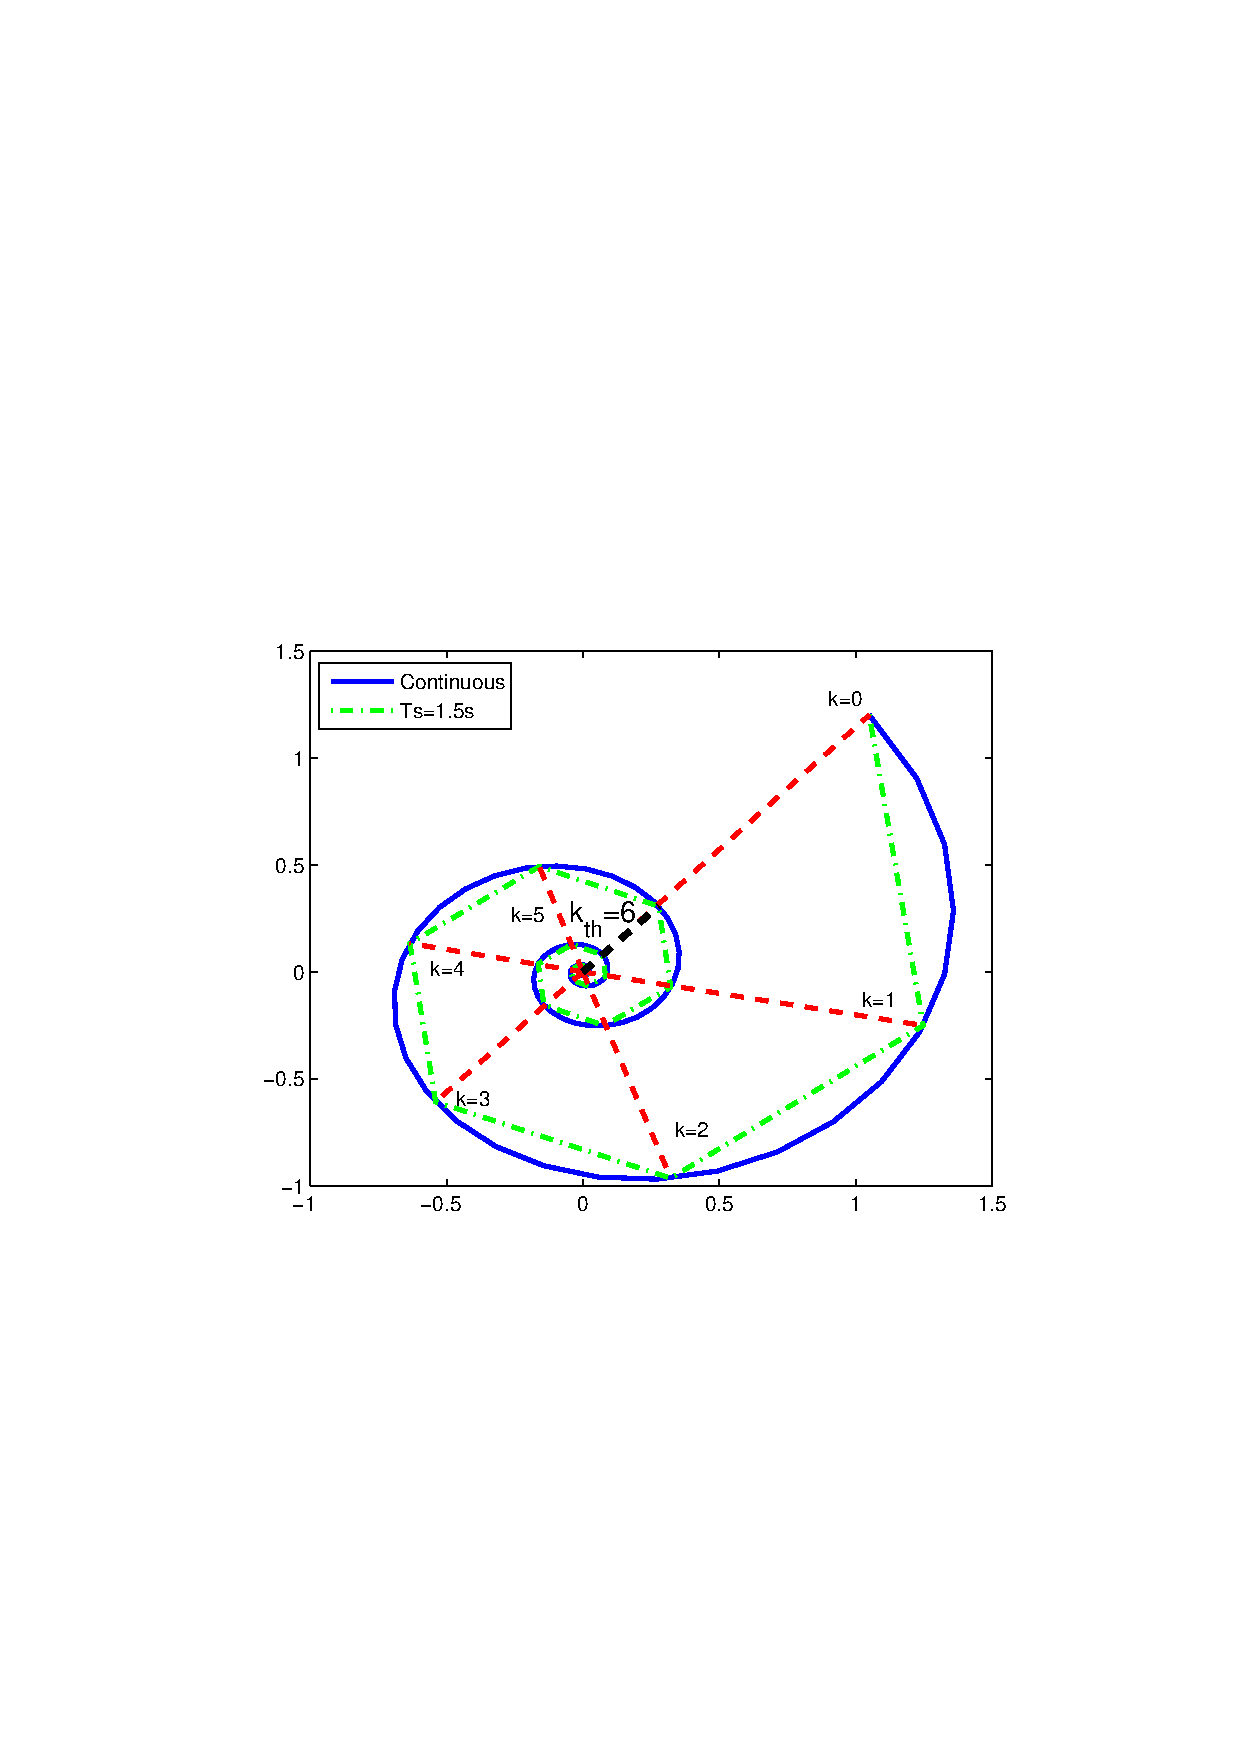
\includegraphics[width=0.6\textwidth]{./figures/ct.pdf}
\vspace{0.1cm}
\label{fig:ct}
\end{figure}
\end{frame}

%\begin{frame}{Illustrative Example}
%We illustrate our approach with an example,
%extracted from the literature~\cite{Franklin15}.
%%
%We start with a candidate solution with all coefficients zero, $K=[0
%  \ 0 \ 0]^T$, and a precision of $I_p=13$, $F_p=3$.  In the first
%{\sc verify} stage, the {\sc safety} check finds the counterexample
%%
%$ x_0 = [-0.5 \ 0.5 \ 0.5] $.
%%
%After adding the new counterexample to its sets of {\sc inputs}, {\sc
%  synthesize} finds the candidate solution $K=[0 \ 0
%  \ 0.00048828125]^T$, which prompts the {\sc safety} verifier to
%return $x_0=[-0.5 -0.5 -0.5]$ as the new counterexample.
%
%In the subsequent iteration, the synthesizer is unable to find further 
%suitable candidates and it returns UNSAT, meaning that the current precision is
%insufficient.  Consequently, we increase the precision to $I_p=17$,
%$F_p=7$.
%%
%Since the previous counterexamples were obtained at lower precision,
%we remove them from the set of counterexamples.  Back in the {\sc
%  synthesize} phase, we re-start the process with a candidate solution
%with all coefficients $0$.  Next, the {\sc safety} verification stage
%provides the first counterexample at higher precision, $x_0=[-0.5
%  \ 0.5 \ 0.5]$ and {\sc synthesize} finds $K=[0 \ 0.01171875
%  \ 0.015625]^T$ as a candidate that eliminates this counterexample.
%However, this candidate triggers the counterexample
%$x_0=[0.5\ -0.5\ -0.5]$ found again by the {\sc safety} verification
%stage.  In the next iteration, we get the candidate $K=[0 \ 0
%  \ -0.015625]$, followed by the counterexample $x_0 = [0.5 \ 0.5
%  \ 0.5]$. Finally, {\sc synthesize} finds the candidate $K=[0.01171875
%  \ -0.013671875 \ -0.013671875]^T$, which is validated as a final
%solution by all verification stages.
%end{frame}

\begin{frame}[fragile]{Abstraction-based CEGIS}
\begin{figure}
\centering
{\scriptsize
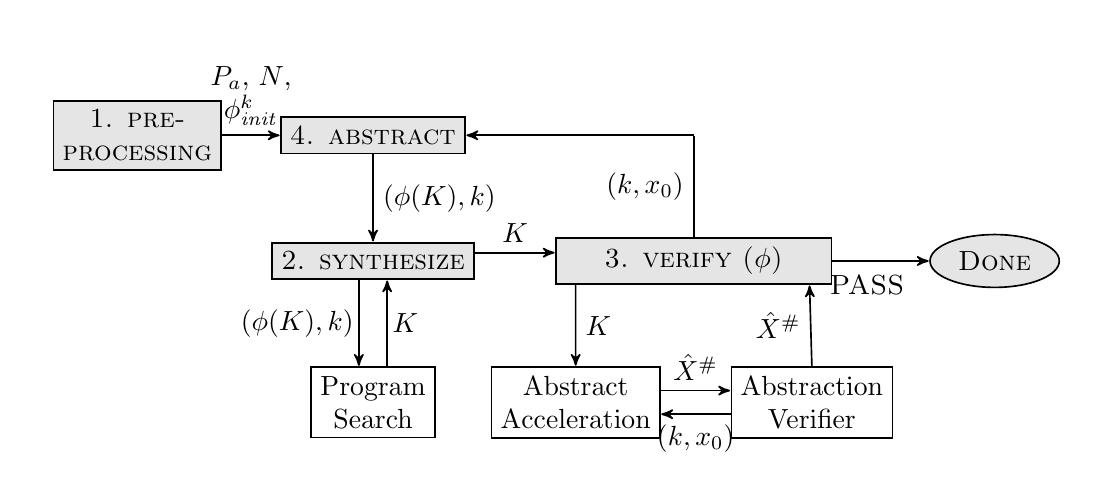
\begin{tikzpicture}[scale=0.3,->,>=stealth',shorten >=.2pt,auto, semithick, ampersand replacement=\&,]
  \matrix[nodes={draw, fill=none, shape=rectangle, minimum height=.2cm, minimum width=.2cm, align=center},row sep=.8cm, column sep=.2cm] {
   \coordinate (aux1);
   \& \coordinate (aux2);
   \& ;\\
   \&\node[fill=gray!20,align=center,xshift=-1.5cm] (pre) {{\sc 1. pre-}\\{\sc processing}};
   \& \node[fill=gray!20,align=center] (abstract) {\sc 4. abstract};
   \& \coordinate (aux); \\ 
   \&
   \& \node[fill=gray!20,align=center] (synth) {\sc 2. synthesize};
   \& \node[fill=gray!20,align=center, minimum width=3.5cm] (verify) {\sc 3. verify ($\phi$)};
      \node[draw=none] (SAT) at ([xshift=2.2cm,yshift=-.3cm]verify)  {\sc PASS};
   \& \node[ellipse, fill=gray!20] (done) {{\sc Done}};\\
   \&
   \& \node[draw,rectangle,align=center] (KSAT) {Program \\ Search};
   \& complexnode/.pic={
     \coordinate (AA);
     \node[draw,rectangle,align=center] (AAV) at ([xshift=-1.5cm]AA.center) {Abstract\\Acceleration};
     \node[draw,rectangle,align=center] (AAC) at ([xshift=1.5cm]AA.center) {Abstraction \\ Verifier};
    }\\
  };
  \path
    (pre.east) edge node[align=center] {$P_a$, $N$,\\ $\phi_\mathit{init}^k$} (abstract.west)
    (abstract.south) edge node{$(\phi(K), k)$} (synth.north)
    ([yshift=1em]synth.east) edge node {$K$} ([yshift=1em]verify.west)
    (aux) edge (abstract.east) 
    (verify.east) edge (done.west);
  \path
    ([xshift=+.6cm]KSAT.north) edge[left] node[xshift=-.3cm] {$(\phi(K),k)$} ([xshift=0.6cm]synth.south) 
    ([xshift=-.6cm]synth.south) edge node[align=center,xshift=.3cm] {$K$} ([xshift=-.6cm]KSAT.north)
    ([yshift=.5cm]AAV.east) edge node{\sl $\hat{X}^\#$} ([yshift=.5cm]AAC.west)
    ([yshift=-.5cm]AAC.west) edge node{$(k,x_0)$} ([yshift=-.5cm]AAV.east)
    (AAC.north) edge node{\sl $\hat{X}^\#$} ([xshift=4.9cm]verify.south)
    ([xshift=-5cm]verify.south) edge node{$K$} (AAV.north);
  \path[-] 
     (verify.north) edge node {$(k,x_0)$} (aux);
\end{tikzpicture}
}
\end{figure}
\end{frame}

\begin{frame}[fragile]{Abstraction-based CEGIS}
\begin{itemize}
\uncover<1->{ \item Calculate $\mat{T}$ such that $P_a = z^n+\sum_{i=1}^p{(a_i-k_i)z^{n-i}}$ is the first line of $\mat{T}\mat{A}_b\mat{T}^{-1}$}
\uncover<2->{\item Calculate $N= \left \{ \nu_1+\nu_2+ \nu_3 \right \}$ from the quantizer resolutions and estimated round-off errors: 

\begin{align*}
\nu_1 \in \left[-\frac{q_1}{2}\ \ \frac{q_1}{2}\right] \wedge \nu_2 \in \left[-\frac{q_2}{2}\ \ \frac{q_2}{2}\right]  \wedge \nu_3 \in \left[-q_3\ \ q_3\right]\nonumber
\end{align*}

where  $q_1$ is the error introduced by the truncation by the ADC, $q_2$ is
the error introduced by the DAC and $q_3$ is the maximum truncation and
rounding error in $u_k=-K \cdot \mathcal{F}_{\langle I_c,F_c \rangle}(x_k)$}

\uncover<3->{
\item Calculate $\phi_\mathit{init}^K := -K x_0 \in \phi_{input} : x_0 \in \phi_{\mathit{init}}$}

\end{itemize}
\end{frame}

%
%\item In the {\sc synthesize} phase, we synthesize a candidate controller

%% Once we have established convergence, we may examine the 
%% safety specification $\phi_{safety}$.
%  $K \in \mathbb{R}\langle I_c,F_c\rangle^n$ that satisfies
%  $\phi_\mathit{stability} \wedge \phi_\mathit{safety} \wedge \phi_\mathit{init}^{K}$ by invoking a SAT solver.
%%%   We obtain it by solving the SAT formula 
%%% $$\mathcal{J}_K=\mathcal{J}\langle I,F \rangle (P_{a-k},\mat{T})\wedge \phi_{safety}$$ 
%%% that satisfies the input constraint and Jury's criteria for 
%%% $P_{a-k}=z^n+\sum_{i=1}^n (a_i-k_i) z^{n-i} : k_i \in \mat{K} \wedge \tilde{\mat{K}}=\mat{K}\mat{T}$,
%%% where $\mathcal{J}\langle I,F \rangle (P,\mat{T})$ is a program describing Jury's method.
%If there is no candidate solution we return UNSAT and exit the loop.
%\item Once we have a candidate solution, we perform a safety verification % If this step fails, we find a counterexample iteration and initial state and create a new constraint to refine our abstraction.
%  %
%  of the 
%  %consisting of evaluating the
%  progression of the system from $\phi_\mathit{init}$ over time,
%$x_{k+1} \models \phi_\mathit{safety}$. %% For this purpose we require 
%%% an initial set $\phi_{init}= x_0 \in [\underline{x_0} \ \overline{x_0}]$ 
%%% from which the system progresses.
%% Obviously, this set $x_0$ 
%% must satisfy the specification; otherwise, the system will be unsafe to begin with.
%% We accept a specification in the form $\mat{E}\mat{T}x_0<\mat{f}$. 
%% The presence of $\mat{T}$ is because this will typically be given in the original 
%% state-space.
%%% Next, we use abstract acceleration to get a second abstraction that 
%  %% encompasses the accelerated continuous reach-tube over an unbounded time.
%  In order to compute the progression of point $x_0$ at iteration $k$,
%  we accelerate the dynamics of the closed-loop system and obtain:
%  %we take the
%  %the closed-loop model:
%  %$x_{k+1}=\mat{A}_{t}x_k+\mat{B}_{n} (\nu_1 + \nu_2 + \nu_3)$
%  %and accelerate it to:
%%
%\begin{align}
%%\label{eq:acc_observer_LTI_cf}
%x=&(A_d-B_dK)^kx_0
%%+\sum_{i=0}^{k-1} \mat{A}_t^i \mat{B}_{t} r_i
%+\sum_{i=0}^{k-1} (A_d-B_dK)^i B_{n}(\nu_1+\nu_2+\nu_3) : B_n= [1\ 1 \cdots \ 1 ]^T
%\end{align}
%%
%As this still requires us to verify the system for every $k$ up to infinity,
%we use abstract acceleration again to obtain the reach-tube, i.e., the set
%of all reachable states at all times given an initial set
%$\phi_\mathit{init}$:
%%
%\begin{align}
%\label{eq:aa_observer_LTI_cf}
%\hat{X}^\#
%=&\mathcal{A} X_0 + \mathcal{B}_{n} N\\
%X_0 =&\left \{x : x \models \phi_\mathit{init} \right\}\nonumber
%\end{align}
%%
%where $\mathcal{A}=\bigcup_{k=1}^\infty (A_d-B_dK)t^k,
%\mathcal{B}_{n}=\bigcup_{k=1}^\infty \sum_{i=0}^k(A_d-B_dK)^iB_{n}$ are
%abstract matrices for the closed-loop system~\cite{cattaruzza2015unbounded},
%whereas the set $N$ is non-deterministically chosen.
%
%We next evaluate $\hat{X}^\# \models \phi_\mathit{safety}$.  If the
%verification holds we have a solution, and exit the loop.  Otherwise, we
%find a counterexample iteration $k$ and corresponding initial point $x_0$
%for which the property does not hold, which we use to locally refine the
%abstraction.  When the abstraction cannot be further refined, we provide
%them to the {\sc abstract} phase.
%%
%%\todo{we should have a better argument here.}
%%\end{enumerate} 
%\item If we reach the {\sc abstract} phase, it means that the candidate solution is not valid,
%  in which case we must refine the abstraction used by the synthesizer.
%\begin{enumerate}
%\item Find the constraints that invalidate the property
% as a set of counterexamples for the eigenvalues, which we define as $\phi_\Lambda$. This is a constraint in the spectrum i.e., transfer function) of the closed loop dynamics. 
%\item We use $\phi_\Lambda$ to
%  further constrain the characteristic polynomial  
%$z^n+\sum_{i=1}^n(a_i-k_i)z^{n-i}=\prod_{i=1}^n (z-\lambda_i) : |\lambda_i|<1 \wedge \lambda_i \models \phi_{\Lambda}$. These constraints correspond to specific iterations for which the system may be unsafe.
%\item Pass the refined abstraction $\phi(K)$ with the new constraints and the list of iterations $k$ to the {\sc synthesize} phase.
%  %, as well as a counterexample plant coefficients ($P_a$) and repeat the loop again. 
%\end{enumerate} 

\begin{frame}{Case Study}
Consider the sampled helicopter example:
\begin{align*}
A_d &= \left[\begin{array}{ccc}2.6207&-1.1793&0.65705\\2&0&0\\0&0.5&0\end{array}\right] &
B_d &= \left [\begin{array}{c}8\\0\\0\end{array}\right]\\
x_0 &\in [-.9\ \ .9] \wedge u \in [-10\ \ 10] \wedge x_k \in [-.92\ \ .92]\\
\mathbb{R}&\langle I,F \rangle=\mathbb{R}\langle 8,8 \rangle
\end{align*}
With pre-processed characteristic polynomial, transform matrix, noise and initial constraints
\begin{align*}
P_a(z) &=z^3 + 2.6207z^2 -2.3586 z + 0.65705\\
T &= \left[\begin{array}{ccc}8&0&0\\0&16&0\\0&0&8\end{array}\right]\\
N &\in [-.00595\ \ .00595]\\
\phi_{init}&=(|K_1|+|K_2|+|K_3|<10.87)
\end{align*}
\end{frame}

\begin{frame}[fragile]{Case Study}
\begin{figure}
\centering
{\scriptsize
\begin{tikzpicture}[scale=0.3,->,>=stealth',shorten >=.2pt,auto, semithick, ampersand replacement=\&,]
  \matrix[nodes={draw, fill=none, shape=rectangle, minimum height=.2cm, minimum width=.2cm, align=center},row sep=1.5cm, column sep=2cm] {
   \coordinate (aux1);
   \& \coordinate (aux2);
   \& ;\\
   \& \node[fill=gray!20,align=center] (abstract) {\sc 4. abstract};
   \& \coordinate (aux); \\ 
   \& \node[fill=gray!20,align=center] (synth) {\sc 2. synthesize};
   \& \node[fill=gray!20,align=center, minimum width=3.5cm] (verify) {\sc 3. verify ($\phi$)};
        \uncover<9>{ \node[draw=none] (SAT) at ([xshift=2.2cm,yshift=-.3cm]verify)  {\sc \textcolor{blue}{PASS}};}

   \\
   \& \node[draw,rectangle,align=center] (KSAT) {Program \\ Search};
   \& complexnode/.pic={
     \coordinate (AA);
     \node[draw,rectangle,align=center] (AAV) at ([xshift=-1.5cm]AA.center) {Abstract\\Acceleration};
     \node[draw,rectangle,align=center] (AAC) at ([xshift=1.5cm]AA.center) {Abstraction \\ Verifier};
    }\\
  };
  \only<1-5>{\path (abstract.south) edge node{$\textcolor{blue}{\begin{array}{c}\phi_{init}^K\\P_a(z)\\k=0\end{array}}$} (synth.north);}
  \only<6->{\path (abstract.south) edge node{$\textcolor{blue}{\begin{array}{c}\phi_{k,x_0}^K\\P_a(z)\\k=0,1,2\end{array}}$} (synth.north);}
    \only<1-2,6>{\path ([yshift=1em]synth.east) edge node {$K$} ([yshift=1em]verify.west);}
    \only<3-5,7->{\path ([yshift=1em]synth.east) edge node {$\textcolor{blue}{K}$} ([yshift=1em]verify.west);}
    \path (aux) edge (abstract.east);
    

  \only<1,6>{\path ([xshift=+.6cm]KSAT.north) edge[left] node[xshift=-.3cm] {$(\phi(K),k)$} ([xshift=0.6cm]synth.south);}
  \only<2-5>{\path ([xshift=+.6cm]KSAT.north) edge[left] node[xshift=-.3cm] {$\textcolor{blue}{\begin{array}{c}\phi_{init}^K\\P_a(z)\end{array}}$} ([xshift=0.6cm]synth.south);}
  \only<7->{\path ([xshift=+.6cm]KSAT.north) edge[left] node[xshift=-.3cm] {$\textcolor{blue}{\begin{array}{c}\phi_{k,x_0}^K\\P_a(z)\\k=0,1,2\end{array}}$} ([xshift=0.6cm]synth.south);}
    \only<1-2,6>{\path ([xshift=-.6cm]synth.south) edge node[align=center,xshift=.3cm] {$K$} ([xshift=-.6cm]KSAT.north);}
    \only<3-5>{\path ([xshift=-.6cm]synth.south) edge node[align=center,xshift=.3cm] {$\textcolor{blue}{\left[\begin{array}{c}0.24609375\\-0.125\\0.1484375\end{array}\right]^T}$} ([xshift=-.6cm]KSAT.north);}
    \only<7->{\path ([xshift=-.6cm]synth.south) edge node[align=center,xshift=.3cm] {$\textcolor{blue}{\left[\begin{array}{c}0.23828125\\-0.17578125\\0.109375\end{array}\right]^T}$} ([xshift=-.6cm]KSAT.north);}
    \only<1-3,6-7>{
    \path ([yshift=.5cm]AAV.east) edge node{\sl $\hat{X}^\#$} ([yshift=.5cm]AAC.west);
    \path ([yshift=-.5cm]AAC.west) edge node{$(k,x_0)$} ([yshift=-.5cm]AAV.east);
    \path (AAC.north) edge node{\sl $\hat{X}^\#$} ([xshift=4.9cm]verify.south);
    \path ([xshift=-5cm]verify.south) edge node{$K$} (AAV.north);
    }
    \only<4-5,8->{
    \path ([yshift=.5cm]AAV.east) edge node{\sl $\textcolor{blue}{\hat{X}^\#}$} ([yshift=.5cm]AAC.west);
    \path ([yshift=-.5cm]AAC.west) edge node{$\textcolor{blue}{(k,x_0)}$} ([yshift=-.5cm]AAV.east);
    \path (AAC.north) edge node{\sl $\textcolor{blue}{\hat{X}^\#}$} ([xshift=4.9cm]verify.south);
    \path ([xshift=-5cm]verify.south) edge node{$\textcolor{blue}{K}$} (AAV.north);
    }
    
  \only<1-4,7->{\path[-] (verify.north) edge node {$(k,x_0)$} (aux);}
  \only<5-6>{\path[-] (verify.north) edge node {$\tiny \textcolor{blue}{\left(\begin{array}{cc}2,&[\begin{array}{ccc}.9&-.9&.9\end{array}]\\3,&[\begin{array}{ccc}.9&-.9&-.9\end{array}]\end{array}\right)}$} (aux);}
\end{tikzpicture}
}
\end{figure}
\end{frame}

\end{document}
